This paragraph will present the two dashboards implemented, the design principles used, and the SA demons that were tried to avoid. As mentioned before, to ensure that most of the requirements identified in the previous stage could be represented, it was decided to use a dataset entirely created by us to have full control over the data and its structure.

The whole system is divided into two dashboards, each associated with multiple goals. The first dashboard aims to estabilish \textbf{Common Operational Picutre} that allows students to have a shared understanding of the current situation by integrating multiple subgoals into coherent visualizations. 
In contrast, the second dashboard, focuses on tracking and presenting student learning progress within a specific course.

\begin{itemize}
    \item \textbf{Dashboard I}: Subgoal 1.2.1 - Improve student engagement with the platform and Subgoal 1.2.2 - Optimize student learning through personalization.
    \item \textbf{Dashboard II}: Subgoal 1.1.1 - Comprehension of the fundamental concepts of cybersecurity and Subgoal 1.2.1 - Improve student engagement with the platform and Subgoal 1.2.2 - Optimize student learning through personalization.
\end{itemize} 

Both of the dashboards attempt to achieve the trade-off between supporting the operator's goal and supporting the overall SA. By placing the most important information appropriately at the center of each dashboard and positioning the supporting information on the sides, we ensure that critical data is easily accessible while still providing a comprehensive view. 

Additionally, the dashboards are designed to be user-friendly, with a clean and intuitive interface that allows students to quickly understand the information presented. This design choice is intended to reduce the cognitive load on the student, making it easier to process the data and make informed decisions, thereby further supporting individual objectives and improving situation awareness.

To limit complexity, and effort has been made to always provide explicit support SA Level 2, where necessary, so that information about his learning progress is always available to the student. In this way, the student can quickly understand his current situation and make informed decisions about his learning path.


\section{Dashboard I}

The subgoals of this dashboard are to not lose the student's engagement with 
the platform and to help in adapting the learning process to the student's
needs. 

To make the student aware that he/she is looking
at the home page of the platform the name \textit{OffSec} is added,
which states for \textit{Offensive Cybersecurity}, that is the field
in which the student has to upskill his/her expertise. To remark that this
dashboard is the home page is added \textit{Welcome Marta!} message.
These two elements help the student to not use the wrong mental model
when he/she has to interpret the elements present inside the dashboard.
In this way, the \textbf{Wrong Mental Model} demon is avoided.

\begin{figure}[H]
    \centering
    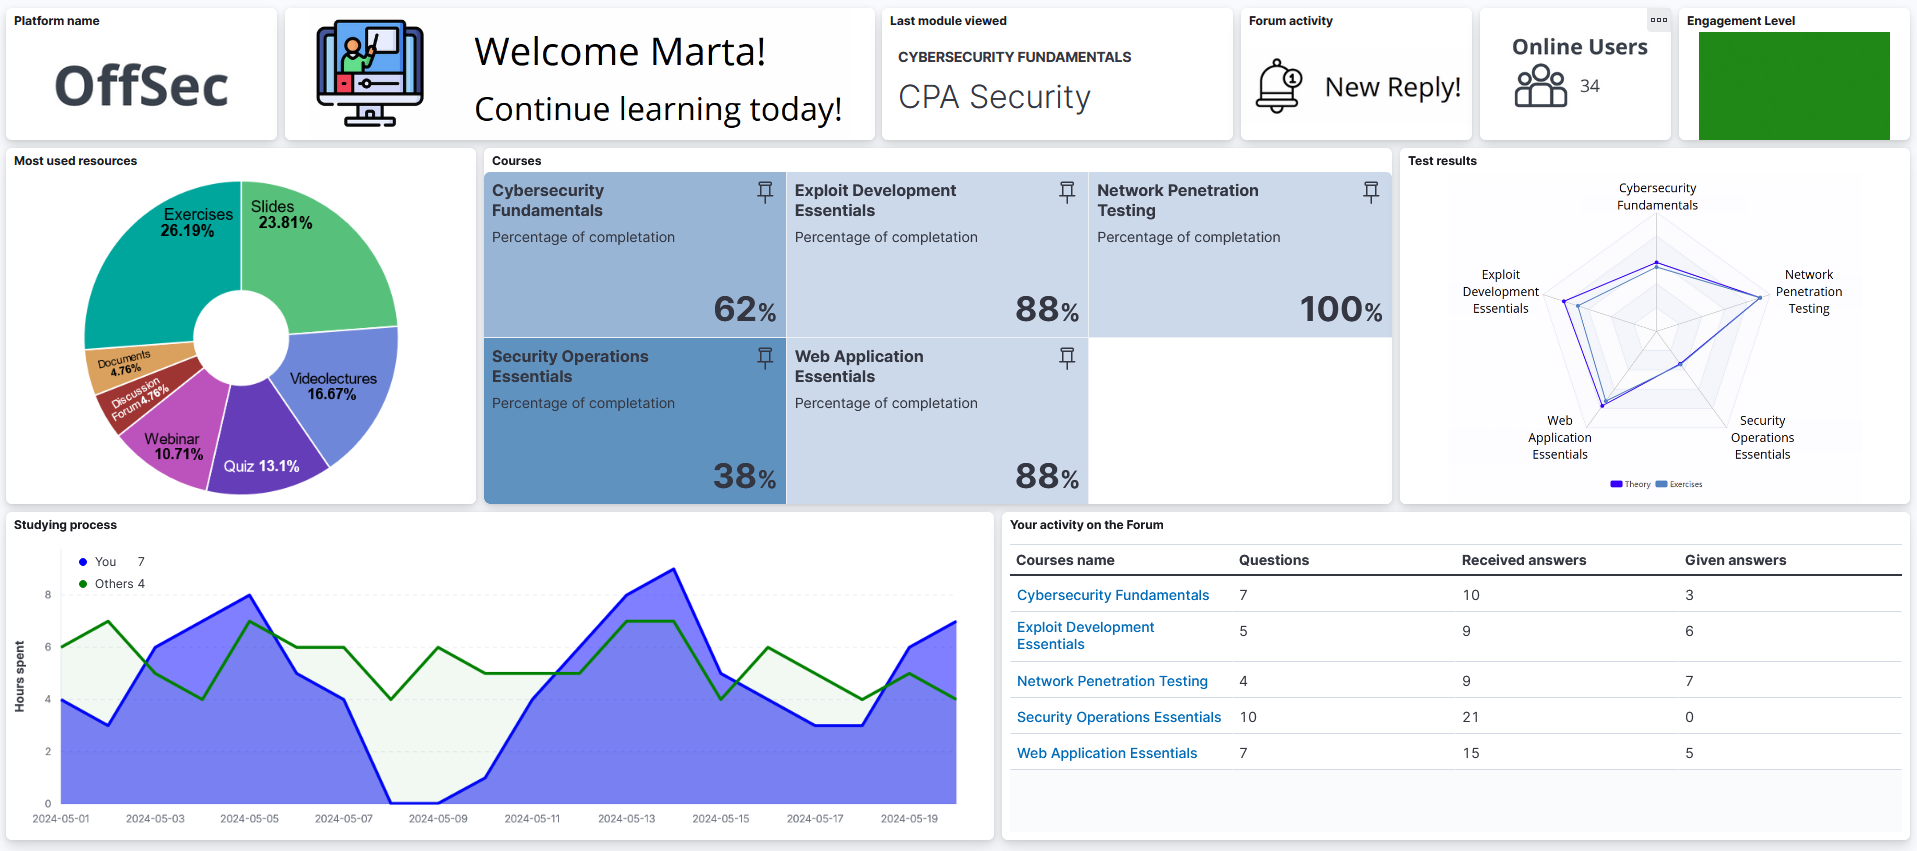
\includegraphics[width=0.9\textwidth]{assets/dashboard_1.png}
    \caption{Dashboard I}
    \label{fig:dashboard_1}
\end{figure}

In order to guarantee the \textbf{Principle 4}, the dashboard should be designed to have the
elements supporting the goals in the middle of the dashboard, surrounded by elements helping the
global picture of the student. But to ensure the dashboard
is coherent with what a student expects to see when he/she visits an e-learning system, as 
can be seen from the previous image, in the middle of the screen is present a matrix containing 
the different courses the student has to complete to upskill himself/herself. In this matrix is 
shown the percentage of completion of each course allowing the student to immediately know his/her
situation, thus supporting the student's global view of his/her situation. Related to this element, hence
helping in forming the right global situation awareness of the student, on 
the right side is present a spider chart showing the results of the student on the theory tests and
the exercises tests, weighted on the number of tests completed for the course.
Instead, on the left side of the screen, is present a
donut chart, which shows how many different resources are available for the different courses 
the student has used, in order to support the \textbf{subgoal 1.2.2}.

The linear graph, which shows the student's time spent on the platform since the start of
the process of upskilling supports the \textbf{subgoal 1.2.1}. Another support to this subgoal
is given by the table containing the activity of the student on the forum, showing how many questions 
the student asked, how many answers received and how many answers the student has given. Both the 
elements are shown in the following figure.

\begin{figure}[H]
    \centering
    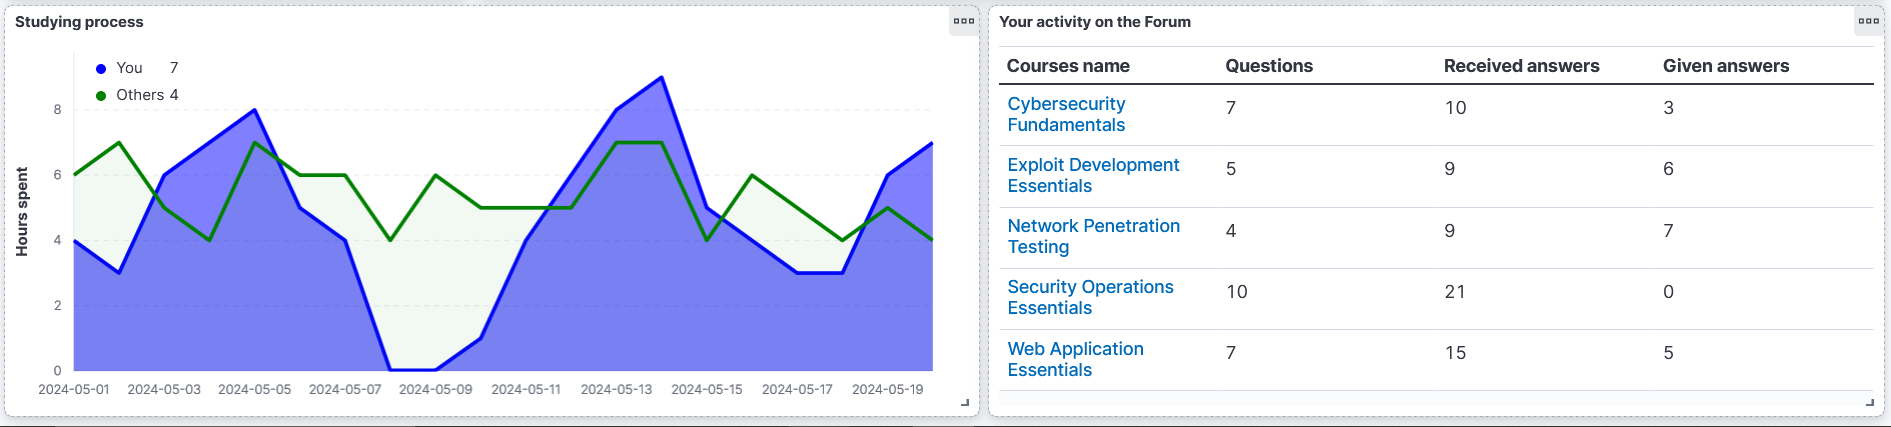
\includegraphics[width=0.9\textwidth]{assets/dashboard_1_121.png}
    \caption{Dashboard I - Subgoal 1.2.1}
    \label{fig:dashboard_1_subgoal_121}
\end{figure}


The remaining part of the dashboard contains different elements that remind the student
situation regarding the subgoals of the first major goal (how he/she is upgrading 
his/her skill). 

\begin{figure}[H]
    \centering
    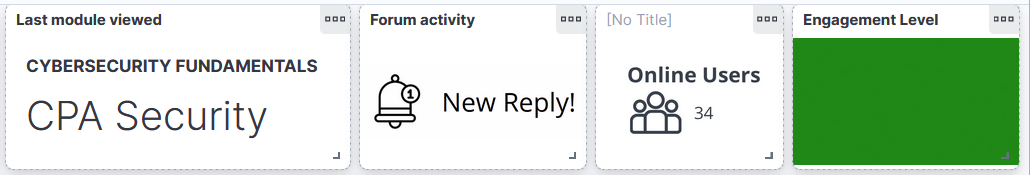
\includegraphics[width=0.9\textwidth]{assets/dashboard_1_globaltop.png}
    \caption{Dashboard I - Global Top}
    \label{fig:dashboard_1_global_top}
\end{figure}

These elements show student engagement with the platform by showing (from right to left)
the level of engagement computed with the CST described in a previous chapter,
how many students are online, a section
where are shown notifications from the forum 
and an element where is present the last viewed module helps the student
to remember what module was viewed last.
All these elements ensure to have the global situation awareness in each moment, 
to avoid the \textbf{Attentional Tunneling} demon. The student is not only focused
on his/her engagement with the platform or his/her state in the learning process but is
also aware of his/her results from all the tests he/she has done until now.

For this dashboard, the \textbf{Principle 1}, the \textbf{Principle 2} and the \textbf{Principle 3}
have been used as base principles to design the different elements. Thanks to that, the 
visualization of the student's goal is easy to find, since the elements are positioned in center-left
part of the screen. 

To support the student's comprehension and avoid the 
\textbf{Memory Trap} demon, the data are processed and integrated: the spider chart
(positioned on the right side) shows in a faster way the results of the student than
could be done with a table. For the same reason, the donut chart allows a clearer 
understanding of which resources the student prefers more. This kind of visualization of the
data helps in reducing the quantity of data to show in the dashboard to 
avoid the \textbf{Data Overload} demon. Consequently, the \textbf{Complexity Creep} demon is not present.

The \textbf{Principle 5} is supported by the element that communicates the number of 
notifications from the forum, which capture the attention of the student and
facilitate the change between goal-driven and data-driven processing. As said before
this element helps in avoiding the \textbf{Attentional Tunneling} demon.

The \textbf{Principle 6} is used to capture the student's attention on the course that
he/she has completed less. In addition to the percentage of completion of the course,
the intensity of the color of the element in the matrix decreases with the increase
of the percentage of completion, then guiding the student toward the course he/she has more to
do before the deadline of the courses. The engagement level element is displayed as a square
shape filled with a color (green, yellow, orange), it can capture the student's attention when is not needed, so 
causing a bit of the \textbf{Salience} demon. But this is not going to cause a
level of stress to reduce the working memory, as can be worse in other scenarios with 
faster dynamics.

In order to not get \textbf{Data Overload} demon, as said before, the data are visualized
more compactly, for example, is not shown the sequence of the votes of the student in
the home dashboard, but is shown a spider graph containing the results of the student on the
theory tests and the exercises tests, weighted on the number of tests completed for the course.

The \textbf{Out of the Loop} demon is not present inside the dashboard, because
the student is aware of his/her situation in the learning process, thanks to the results of each
test done until now, how many tests he/she has done. In addition, there is not any 
element that can work alone, without the intervention of the student, because in the 
learning process has to be the student to decide what to do and when to do it.

Regarding level three of
Situation Awareness, the linear graph helps the student to project the time he/she will
spend on the platform in the future on the base of the actual trend.

\section{Dashboard II}

The goal of the dashboard is to support the operator's objective of understanding the student's learning progress within a specific course. It is characterized by a title \textbf{Cybersecurity Fundamentals} to indicate the course the student is currently focusing on. The inclusion of a specific course title on the dashboard plays a crucial role in preventing user confusion, especially given the variety of courses a student might be enrolled in. 

This clear indication of the course focus helps to avoid the misinterpretation of information, which is particularly important under conditions of high environmental or emotional stress. By doing so, it directly addresses and mitigates the risk of the \textbf{Wrong Mental Model} demon, ensuring that students maintain an accurate understanding of their learning progress and requirements within the context of the specific course they are viewing. 

Some common guidelines were used to blend the user experience and create a sense of confidence in switching between the different dashboards and to enhance efficiency by transporting the experience matured in one dashboard to the other. This is helpful so that the operator can create expectations about the interface, increasing his or her satisfaction.


Principle 8 guided the design of the entire dashboard, since information is not shown as it is obtained in order to avoid the \textbf{Data Overload} demon since it can increase the complexity of the dashboard and make it difficult to have a comprehensive understanding of the situation.
The choice of different data visualizations used made it possible to reduce the effects of the \textbf{Data Overload} demon as well, by being able to convey the same information by expressing it in graphical form rather than in textual or tabular form (e.g., pie charts for the most used resources), reducing the cognitive load on the student. 

A first view of the second dashboard is shown in the following figure.

\begin{figure}[H]
    \centering
    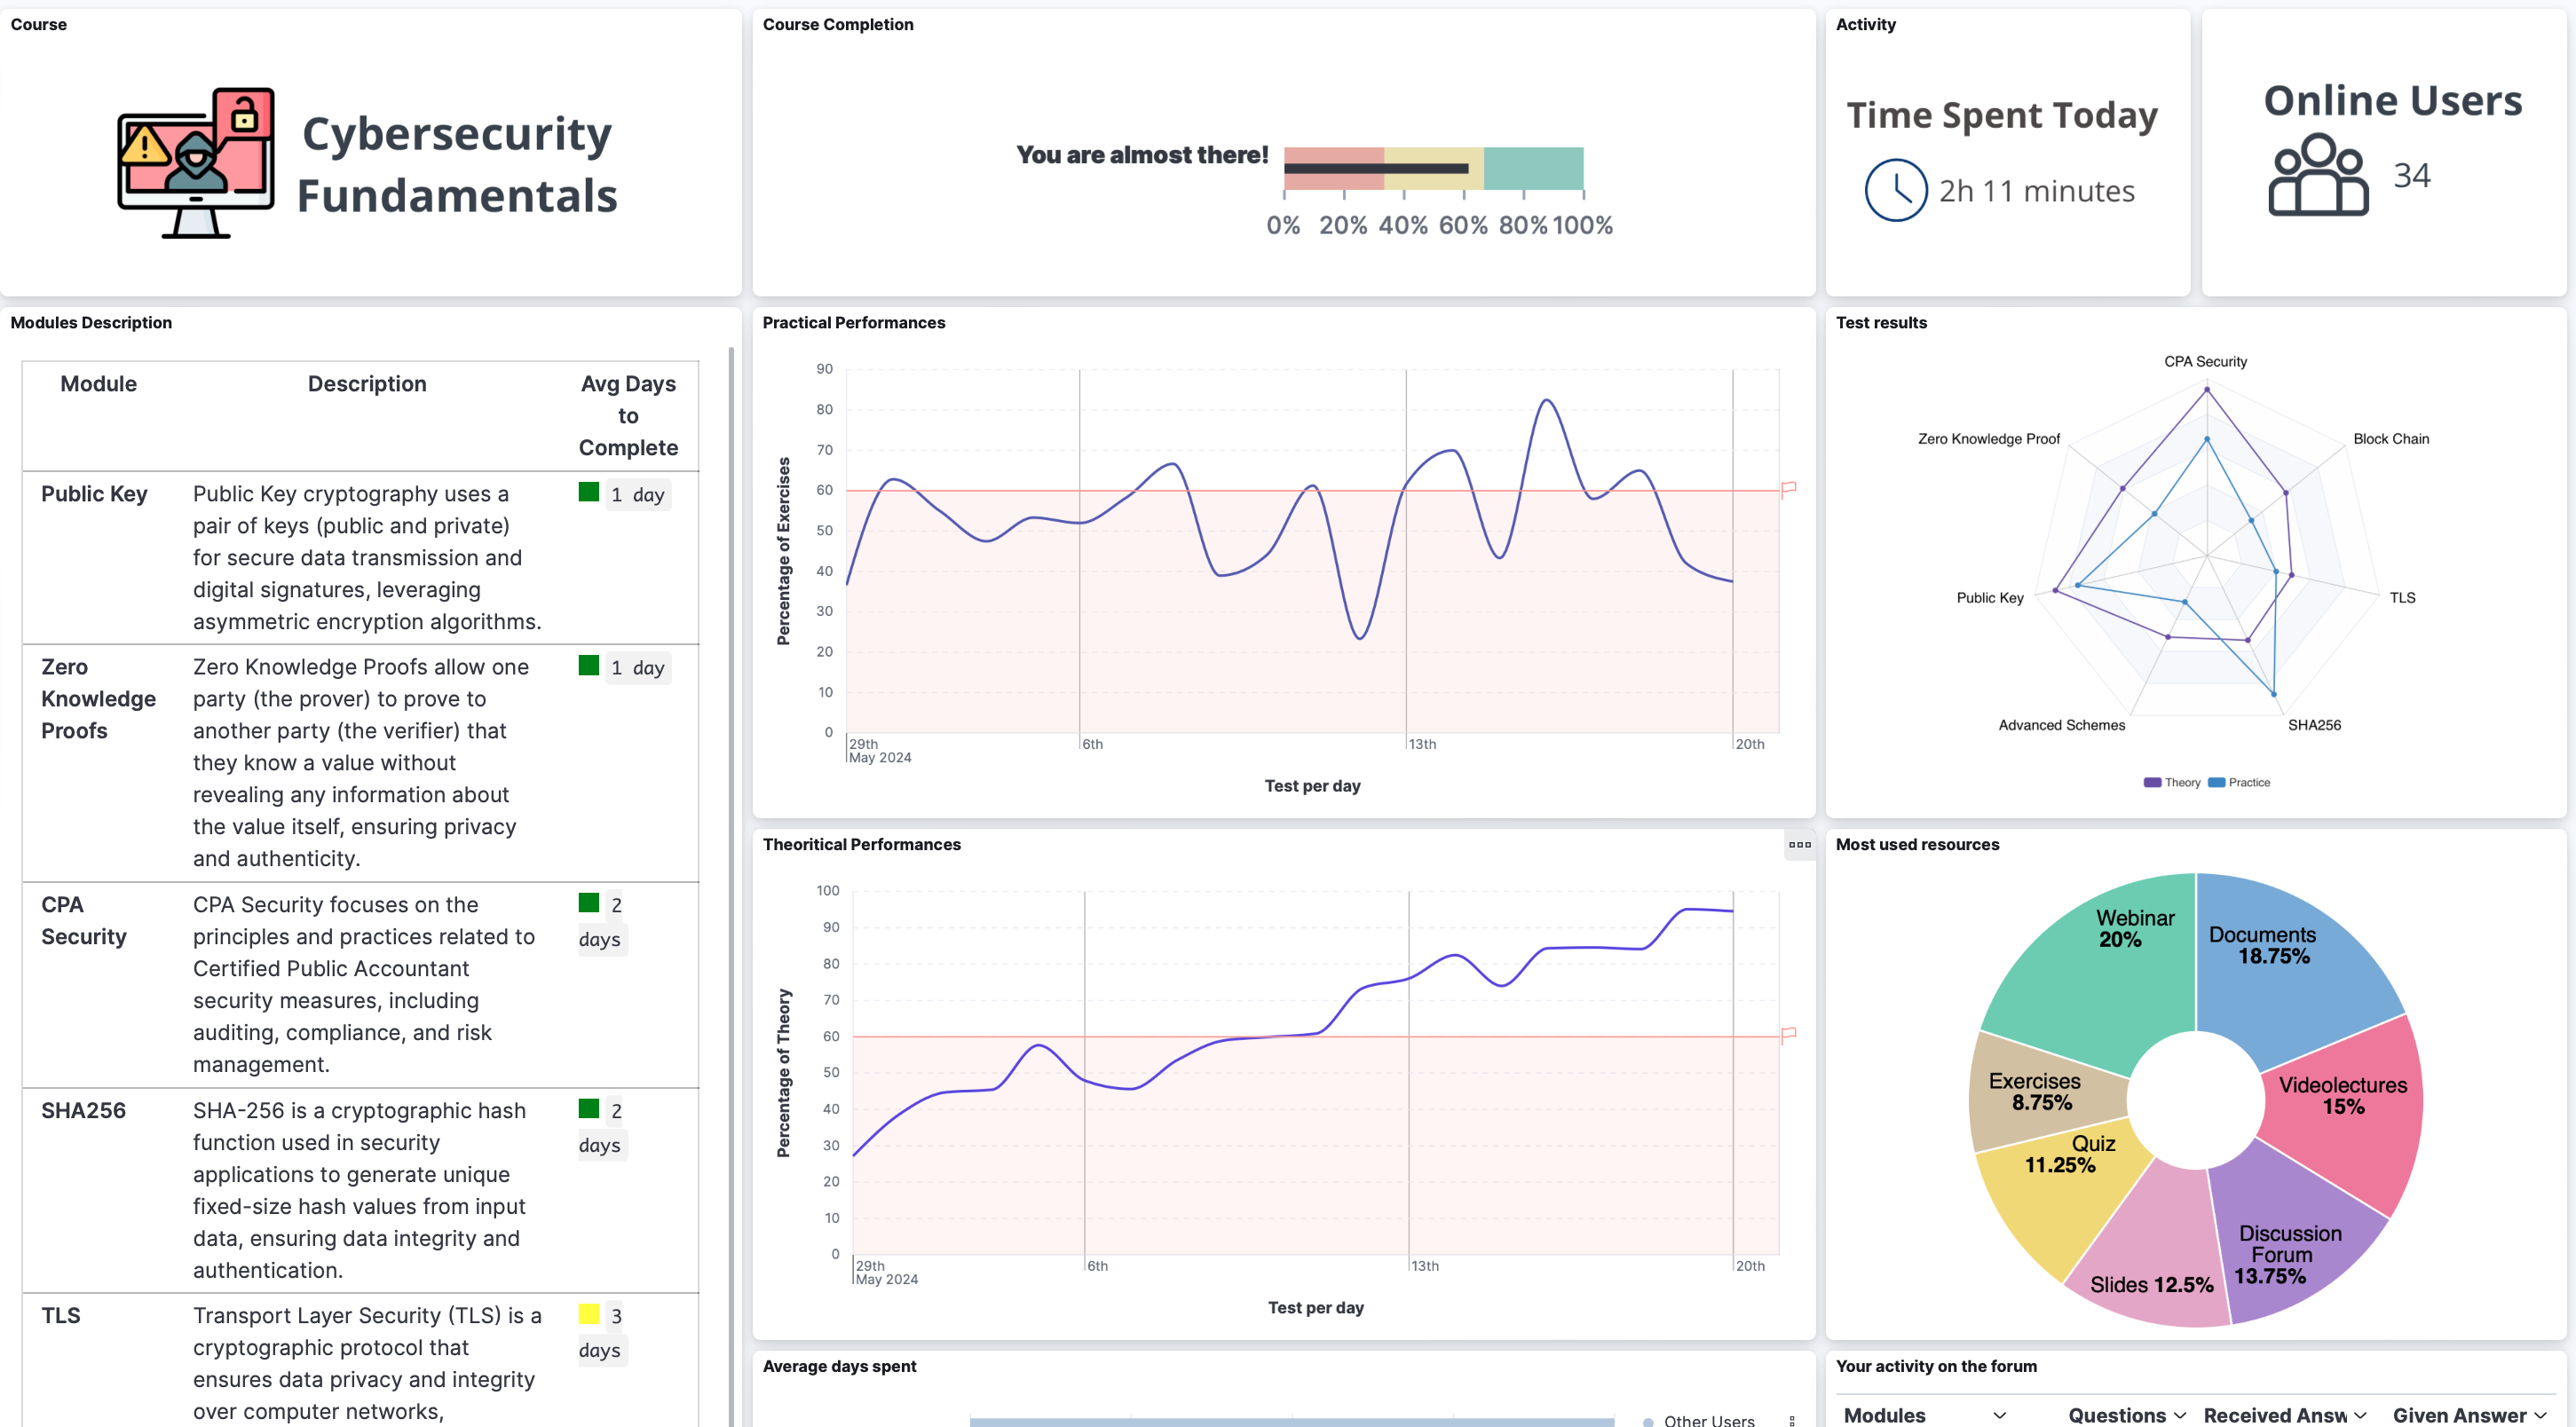
\includegraphics[width=0.9\textwidth]{assets/dashboard_2.png}
    \caption{Dashboard II}
    \label{fig:dashboard_2}
\end{figure}

With multiple subgoals active on the dashboard, it’s important that when a student opens it, they can quickly figure out the necessary information to achieve their objectives. 

This follows \textbf{Design Principle 1}, which ensures that information is provided effectively to support decision-making. When a student clicks on a course, they will see charts in the center of the dashboard showing their progress and course completion status.

These charts, like the others on the dashboard, also satisfy \textbf{Design Principle 2} because the interface provides already processed and integrated information at level 2. Specifically, the data levels (level 2 and level 1) allow for a complete understanding of a critical situation, such as the student's performance in the course, without the need for further processing.

To ensure that salience is appropriately balanced within the dashboard, emphasis is placed only on information considered important. For instance, the red threshold line in the main charts indicates that if a student's end-of-module test scores fall below 60\%, they need to decide on a strategy for improvement. This visual cue helps students understand that they should aim for scores above this threshold.

Additionally, the estimated completion days for each module, where all the modules are listed with their description, are highlighted in red if they exceed four days, based on data from previous users who have taken the course. This alerts students that they may need to put in more effort for these particular modules.
The use of red to draw attention to critical areas complies with Design Principle 6, clearly signaling to the student where they need to focus and prompting them to take corrective action if necessary.

The dashboard also includes a gauge chart dedicated to overall course completion. If a student has completed less than 40\% of the course, this chart will highlight the need for increased attention to ensure timely course completion.
The addition of a course completion chart helps reduce the cognitive load on users by offering a visual depiction of their progress. This feature was intentionally introduced to prevent users from having to remember the completion percentage shown on the main dashboard. By replicating this information across subsequent dashboards, our goal is to overcome the challenge of relying on memory (facing the Memory Trap demon), which can often not guarantee accurate awareness and decision-making.

These design choices also support \textbf{Design Principle 3} by providing level 3 projection assistance. This means that if a student maintains consistent performance across multiple modules, it can be projected that they will likely perform well in future modules. 

Given that the dashboard supports three subgoals, it is likely that when a student first opens the dashboard for a specific course, they do so to check their understanding of the fundamental cybersecurity concepts. Through various charts—such as those showing their theoretical and practical test performance, course completion status, and average grades, they can assess their level of understanding of the course. 
This also supports the subgoal related to optimizing learning through personalization, including a pie chart that shows the usage of different learning materials for each module in order to show a student learning preferences. 

The other charts support goals related to engagement with the platform. For example, these include activities in the forum, engagement level badges obtained from the CST, the number of users online at the time of access, the time spent on the platform, and the days taken to complete each module compared to other students.

Therefore, we assume that at first glance, the student decides to focus on the first subgoal \textbf{Comprehension of the fundamental concepts of cybersecurity} to reach their objective and then potentially switches to other supported goals as they shift their attention to the other charts. This approach satisfies Design Principle 5 and Design Principle 4 by including elements in the dashboard that capture attention on aspects satisfying different goals. This prevents attention from being confined to a limited set of information, thereby overcoming the issue of attentional tunneling and supporting the switch between goal-driven and data-driven modes based on the goal the student wishes to achieve.

